\documentclass[12pt, twoside]{article}
\usepackage[letterpaper, margin=1in, headsep=0.5in]{geometry}
\usepackage[english]{babel}
\usepackage[utf8]{inputenc}
\usepackage{amsmath}
\usepackage{amsfonts}
\usepackage{amssymb}
\usepackage{tikz}
%\usetikzlibrary{quotes, angles}

\usepackage{graphicx}
\usepackage{enumitem}
\usepackage{multicol}

\usepackage{fancyhdr}
\pagestyle{fancy}
\fancyhf{}
\renewcommand{\headrulewidth}{0pt} % disable the underline of the header

\fancyhead[RE]{\thepage}
\fancyhead[RO]{\thepage \\ Name: \hspace{3cm}}
\fancyhead[L]{BECA / Dr. Huson / 10th Grade Geometry\\* Unit 8 Transformations\\12 March 2019}

\begin{document}
\subsubsection*{8-6 Do Now: Transformation compositions}
  \begin{enumerate}


  \item Quadrilateral $ABCD$ undergoes two tranformations mapping it onto $A''B''C''D''$, as shown below. Specify the two tranformations in order. Complete a table showing the coordinates of the translated points.\\[1cm]
   \hspace{1cm} $A(-5,-1) \rightarrow$\\[0.7cm]
   \hspace{1cm} $B(-5,4) \rightarrow$\\[0.7cm]
   \hspace{1cm} $C(0,3) \rightarrow$\\[0.7cm]
   \hspace{1cm} $D(-2,-1) \rightarrow$

    \vspace{0.5cm}

      \begin{center} %4 quadrant regents grid w T-Chart
      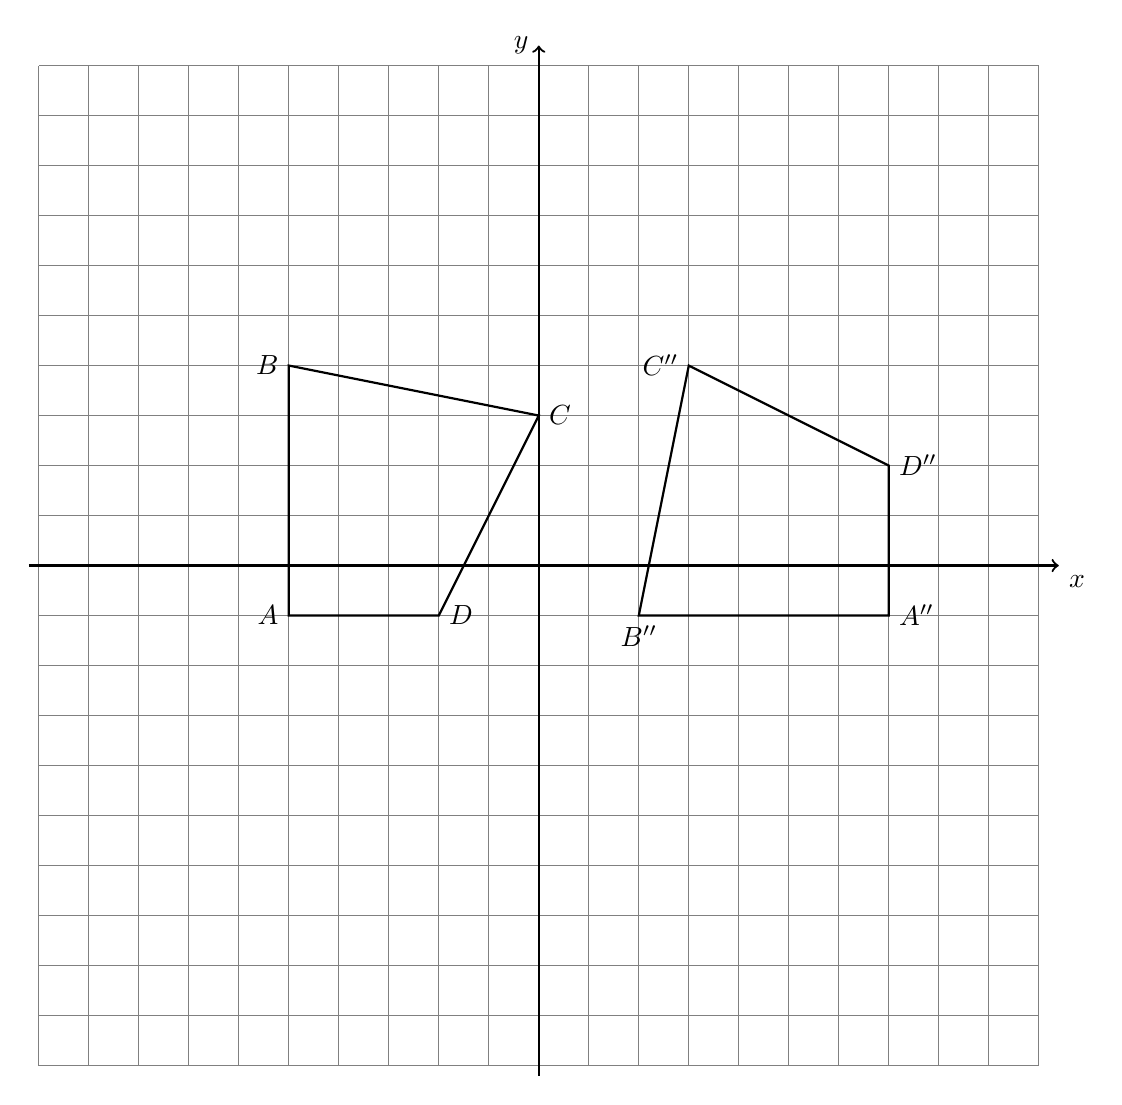
\begin{tikzpicture}[scale=.635]
        \draw [help lines] (-10,-10) grid (10,10);
        \draw [thick, ->] (-10.2,0) -- (10.4,0) node [below right] {$x$};
        \draw [thick, ->] (0,-10.2)--(0,10.4) node [left] {$y$};
        \draw [thick] (-5,-1)node[left]{$A$}--
          (-5,4)node[left]{$B$}--
          (0,3)node[right]{$C$}--
          (-2,-1)node[right]{$D$}--cycle;
        \draw [thick] (7,-1)node[right]{$A''$}--
          (2,-1)node[below]{$B''$}--
          (3,4)node[left]{$C''$}--
          (7,2)node[right]{$D''$}--cycle;
      \end{tikzpicture}
      \end{center}

  \end{enumerate}

  \end{document}
